% !TeX program = pdflatex
\documentclass{article}
\usepackage{iclr2027_conference,times}

%%%%% NEW MATH DEFINITIONS %%%%%

\usepackage{amsmath,amsfonts,bm}

% Mark sections of captions for referring to divisions of figures
\newcommand{\figleft}{{\em (Left)}}
\newcommand{\figcenter}{{\em (Center)}}
\newcommand{\figright}{{\em (Right)}}
\newcommand{\figtop}{{\em (Top)}}
\newcommand{\figbottom}{{\em (Bottom)}}
\newcommand{\captiona}{{\em (a)}}
\newcommand{\captionb}{{\em (b)}}
\newcommand{\captionc}{{\em (c)}}
\newcommand{\captiond}{{\em (d)}}

% Highlight a newly defined term
\newcommand{\newterm}[1]{{\bf #1}}


% Figure reference, lower-case.
\def\figref#1{figure~\ref{#1}}
% Figure reference, capital. For start of sentence
\def\Figref#1{Figure~\ref{#1}}
\def\twofigref#1#2{figures \ref{#1} and \ref{#2}}
\def\quadfigref#1#2#3#4{figures \ref{#1}, \ref{#2}, \ref{#3} and \ref{#4}}
% Section reference, lower-case.
\def\secref#1{section~\ref{#1}}
% Section reference, capital.
\def\Secref#1{Section~\ref{#1}}
% Reference to two sections.
\def\twosecrefs#1#2{sections \ref{#1} and \ref{#2}}
% Reference to three sections.
\def\secrefs#1#2#3{sections \ref{#1}, \ref{#2} and \ref{#3}}
% Reference to an equation, lower-case.
\def\eqref#1{equation~\ref{#1}}
% Reference to an equation, upper case
\def\Eqref#1{Equation~\ref{#1}}
% A raw reference to an equation---avoid using if possible
\def\plaineqref#1{\ref{#1}}
% Reference to a chapter, lower-case.
\def\chapref#1{chapter~\ref{#1}}
% Reference to an equation, upper case.
\def\Chapref#1{Chapter~\ref{#1}}
% Reference to a range of chapters
\def\rangechapref#1#2{chapters\ref{#1}--\ref{#2}}
% Reference to an algorithm, lower-case.
\def\algref#1{algorithm~\ref{#1}}
% Reference to an algorithm, upper case.
\def\Algref#1{Algorithm~\ref{#1}}
\def\twoalgref#1#2{algorithms \ref{#1} and \ref{#2}}
\def\Twoalgref#1#2{Algorithms \ref{#1} and \ref{#2}}
% Reference to a part, lower case
\def\partref#1{part~\ref{#1}}
% Reference to a part, upper case
\def\Partref#1{Part~\ref{#1}}
\def\twopartref#1#2{parts \ref{#1} and \ref{#2}}

\def\ceil#1{\lceil #1 \rceil}
\def\floor#1{\lfloor #1 \rfloor}
\def\1{\bm{1}}
\newcommand{\train}{\mathcal{D}}
\newcommand{\valid}{\mathcal{D_{\mathrm{valid}}}}
\newcommand{\test}{\mathcal{D_{\mathrm{test}}}}

\def\eps{{\epsilon}}


% Random variables
\def\reta{{\textnormal{$\eta$}}}
\def\ra{{\textnormal{a}}}
\def\rb{{\textnormal{b}}}
\def\rc{{\textnormal{c}}}
\def\rd{{\textnormal{d}}}
\def\re{{\textnormal{e}}}
\def\rf{{\textnormal{f}}}
\def\rg{{\textnormal{g}}}
\def\rh{{\textnormal{h}}}
\def\ri{{\textnormal{i}}}
\def\rj{{\textnormal{j}}}
\def\rk{{\textnormal{k}}}
\def\rl{{\textnormal{l}}}
% rm is already a command, just don't name any random variables m
\def\rn{{\textnormal{n}}}
\def\ro{{\textnormal{o}}}
\def\rp{{\textnormal{p}}}
\def\rq{{\textnormal{q}}}
\def\rr{{\textnormal{r}}}
\def\rs{{\textnormal{s}}}
\def\rt{{\textnormal{t}}}
\def\ru{{\textnormal{u}}}
\def\rv{{\textnormal{v}}}
\def\rw{{\textnormal{w}}}
\def\rx{{\textnormal{x}}}
\def\ry{{\textnormal{y}}}
\def\rz{{\textnormal{z}}}

% Random vectors
\def\rvepsilon{{\mathbf{\epsilon}}}
\def\rvtheta{{\mathbf{\theta}}}
\def\rva{{\mathbf{a}}}
\def\rvb{{\mathbf{b}}}
\def\rvc{{\mathbf{c}}}
\def\rvd{{\mathbf{d}}}
\def\rve{{\mathbf{e}}}
\def\rvf{{\mathbf{f}}}
\def\rvg{{\mathbf{g}}}
\def\rvh{{\mathbf{h}}}
\def\rvu{{\mathbf{i}}}
\def\rvj{{\mathbf{j}}}
\def\rvk{{\mathbf{k}}}
\def\rvl{{\mathbf{l}}}
\def\rvm{{\mathbf{m}}}
\def\rvn{{\mathbf{n}}}
\def\rvo{{\mathbf{o}}}
\def\rvp{{\mathbf{p}}}
\def\rvq{{\mathbf{q}}}
\def\rvr{{\mathbf{r}}}
\def\rvs{{\mathbf{s}}}
\def\rvt{{\mathbf{t}}}
\def\rvu{{\mathbf{u}}}
\def\rvv{{\mathbf{v}}}
\def\rvw{{\mathbf{w}}}
\def\rvx{{\mathbf{x}}}
\def\rvy{{\mathbf{y}}}
\def\rvz{{\mathbf{z}}}

% Elements of random vectors
\def\erva{{\textnormal{a}}}
\def\ervb{{\textnormal{b}}}
\def\ervc{{\textnormal{c}}}
\def\ervd{{\textnormal{d}}}
\def\erve{{\textnormal{e}}}
\def\ervf{{\textnormal{f}}}
\def\ervg{{\textnormal{g}}}
\def\ervh{{\textnormal{h}}}
\def\ervi{{\textnormal{i}}}
\def\ervj{{\textnormal{j}}}
\def\ervk{{\textnormal{k}}}
\def\ervl{{\textnormal{l}}}
\def\ervm{{\textnormal{m}}}
\def\ervn{{\textnormal{n}}}
\def\ervo{{\textnormal{o}}}
\def\ervp{{\textnormal{p}}}
\def\ervq{{\textnormal{q}}}
\def\ervr{{\textnormal{r}}}
\def\ervs{{\textnormal{s}}}
\def\ervt{{\textnormal{t}}}
\def\ervu{{\textnormal{u}}}
\def\ervv{{\textnormal{v}}}
\def\ervw{{\textnormal{w}}}
\def\ervx{{\textnormal{x}}}
\def\ervy{{\textnormal{y}}}
\def\ervz{{\textnormal{z}}}

% Random matrices
\def\rmA{{\mathbf{A}}}
\def\rmB{{\mathbf{B}}}
\def\rmC{{\mathbf{C}}}
\def\rmD{{\mathbf{D}}}
\def\rmE{{\mathbf{E}}}
\def\rmF{{\mathbf{F}}}
\def\rmG{{\mathbf{G}}}
\def\rmH{{\mathbf{H}}}
\def\rmI{{\mathbf{I}}}
\def\rmJ{{\mathbf{J}}}
\def\rmK{{\mathbf{K}}}
\def\rmL{{\mathbf{L}}}
\def\rmM{{\mathbf{M}}}
\def\rmN{{\mathbf{N}}}
\def\rmO{{\mathbf{O}}}
\def\rmP{{\mathbf{P}}}
\def\rmQ{{\mathbf{Q}}}
\def\rmR{{\mathbf{R}}}
\def\rmS{{\mathbf{S}}}
\def\rmT{{\mathbf{T}}}
\def\rmU{{\mathbf{U}}}
\def\rmV{{\mathbf{V}}}
\def\rmW{{\mathbf{W}}}
\def\rmX{{\mathbf{X}}}
\def\rmY{{\mathbf{Y}}}
\def\rmZ{{\mathbf{Z}}}

% Elements of random matrices
\def\ermA{{\textnormal{A}}}
\def\ermB{{\textnormal{B}}}
\def\ermC{{\textnormal{C}}}
\def\ermD{{\textnormal{D}}}
\def\ermE{{\textnormal{E}}}
\def\ermF{{\textnormal{F}}}
\def\ermG{{\textnormal{G}}}
\def\ermH{{\textnormal{H}}}
\def\ermI{{\textnormal{I}}}
\def\ermJ{{\textnormal{J}}}
\def\ermK{{\textnormal{K}}}
\def\ermL{{\textnormal{L}}}
\def\ermM{{\textnormal{M}}}
\def\ermN{{\textnormal{N}}}
\def\ermO{{\textnormal{O}}}
\def\ermP{{\textnormal{P}}}
\def\ermQ{{\textnormal{Q}}}
\def\ermR{{\textnormal{R}}}
\def\ermS{{\textnormal{S}}}
\def\ermT{{\textnormal{T}}}
\def\ermU{{\textnormal{U}}}
\def\ermV{{\textnormal{V}}}
\def\ermW{{\textnormal{W}}}
\def\ermX{{\textnormal{X}}}
\def\ermY{{\textnormal{Y}}}
\def\ermZ{{\textnormal{Z}}}

% Vectors
\def\vzero{{\bm{0}}}
\def\vone{{\bm{1}}}
\def\vmu{{\bm{\mu}}}
\def\vtheta{{\bm{\theta}}}
\def\va{{\bm{a}}}
\def\vb{{\bm{b}}}
\def\vc{{\bm{c}}}
\def\vd{{\bm{d}}}
\def\ve{{\bm{e}}}
\def\vf{{\bm{f}}}
\def\vg{{\bm{g}}}
\def\vh{{\bm{h}}}
\def\vi{{\bm{i}}}
\def\vj{{\bm{j}}}
\def\vk{{\bm{k}}}
\def\vl{{\bm{l}}}
\def\vm{{\bm{m}}}
\def\vn{{\bm{n}}}
\def\vo{{\bm{o}}}
\def\vp{{\bm{p}}}
\def\vq{{\bm{q}}}
\def\vr{{\bm{r}}}
\def\vs{{\bm{s}}}
\def\vt{{\bm{t}}}
\def\vu{{\bm{u}}}
\def\vv{{\bm{v}}}
\def\vw{{\bm{w}}}
\def\vx{{\bm{x}}}
\def\vy{{\bm{y}}}
\def\vz{{\bm{z}}}

% Elements of vectors
\def\evalpha{{\alpha}}
\def\evbeta{{\beta}}
\def\evepsilon{{\epsilon}}
\def\evlambda{{\lambda}}
\def\evomega{{\omega}}
\def\evmu{{\mu}}
\def\evpsi{{\psi}}
\def\evsigma{{\sigma}}
\def\evtheta{{\theta}}
\def\eva{{a}}
\def\evb{{b}}
\def\evc{{c}}
\def\evd{{d}}
\def\eve{{e}}
\def\evf{{f}}
\def\evg{{g}}
\def\evh{{h}}
\def\evi{{i}}
\def\evj{{j}}
\def\evk{{k}}
\def\evl{{l}}
\def\evm{{m}}
\def\evn{{n}}
\def\evo{{o}}
\def\evp{{p}}
\def\evq{{q}}
\def\evr{{r}}
\def\evs{{s}}
\def\evt{{t}}
\def\evu{{u}}
\def\evv{{v}}
\def\evw{{w}}
\def\evx{{x}}
\def\evy{{y}}
\def\evz{{z}}

% Matrix
\def\mA{{\bm{A}}}
\def\mB{{\bm{B}}}
\def\mC{{\bm{C}}}
\def\mD{{\bm{D}}}
\def\mE{{\bm{E}}}
\def\mF{{\bm{F}}}
\def\mG{{\bm{G}}}
\def\mH{{\bm{H}}}
\def\mI{{\bm{I}}}
\def\mJ{{\bm{J}}}
\def\mK{{\bm{K}}}
\def\mL{{\bm{L}}}
\def\mM{{\bm{M}}}
\def\mN{{\bm{N}}}
\def\mO{{\bm{O}}}
\def\mP{{\bm{P}}}
\def\mQ{{\bm{Q}}}
\def\mR{{\bm{R}}}
\def\mS{{\bm{S}}}
\def\mT{{\bm{T}}}
\def\mU{{\bm{U}}}
\def\mV{{\bm{V}}}
\def\mW{{\bm{W}}}
\def\mX{{\bm{X}}}
\def\mY{{\bm{Y}}}
\def\mZ{{\bm{Z}}}
\def\mBeta{{\bm{\beta}}}
\def\mPhi{{\bm{\Phi}}}
\def\mLambda{{\bm{\Lambda}}}
\def\mSigma{{\bm{\Sigma}}}

% Tensor
\DeclareMathAlphabet{\mathsfit}{\encodingdefault}{\sfdefault}{m}{sl}
\SetMathAlphabet{\mathsfit}{bold}{\encodingdefault}{\sfdefault}{bx}{n}
\newcommand{\tens}[1]{\bm{\mathsfit{#1}}}
\def\tA{{\tens{A}}}
\def\tB{{\tens{B}}}
\def\tC{{\tens{C}}}
\def\tD{{\tens{D}}}
\def\tE{{\tens{E}}}
\def\tF{{\tens{F}}}
\def\tG{{\tens{G}}}
\def\tH{{\tens{H}}}
\def\tI{{\tens{I}}}
\def\tJ{{\tens{J}}}
\def\tK{{\tens{K}}}
\def\tL{{\tens{L}}}
\def\tM{{\tens{M}}}
\def\tN{{\tens{N}}}
\def\tO{{\tens{O}}}
\def\tP{{\tens{P}}}
\def\tQ{{\tens{Q}}}
\def\tR{{\tens{R}}}
\def\tS{{\tens{S}}}
\def\tT{{\tens{T}}}
\def\tU{{\tens{U}}}
\def\tV{{\tens{V}}}
\def\tW{{\tens{W}}}
\def\tX{{\tens{X}}}
\def\tY{{\tens{Y}}}
\def\tZ{{\tens{Z}}}


% Graph
\def\gA{{\mathcal{A}}}
\def\gB{{\mathcal{B}}}
\def\gC{{\mathcal{C}}}
\def\gD{{\mathcal{D}}}
\def\gE{{\mathcal{E}}}
\def\gF{{\mathcal{F}}}
\def\gG{{\mathcal{G}}}
\def\gH{{\mathcal{H}}}
\def\gI{{\mathcal{I}}}
\def\gJ{{\mathcal{J}}}
\def\gK{{\mathcal{K}}}
\def\gL{{\mathcal{L}}}
\def\gM{{\mathcal{M}}}
\def\gN{{\mathcal{N}}}
\def\gO{{\mathcal{O}}}
\def\gP{{\mathcal{P}}}
\def\gQ{{\mathcal{Q}}}
\def\gR{{\mathcal{R}}}
\def\gS{{\mathcal{S}}}
\def\gT{{\mathcal{T}}}
\def\gU{{\mathcal{U}}}
\def\gV{{\mathcal{V}}}
\def\gW{{\mathcal{W}}}
\def\gX{{\mathcal{X}}}
\def\gY{{\mathcal{Y}}}
\def\gZ{{\mathcal{Z}}}

% Sets
\def\sA{{\mathbb{A}}}
\def\sB{{\mathbb{B}}}
\def\sC{{\mathbb{C}}}
\def\sD{{\mathbb{D}}}
% Don't use a set called E, because this would be the same as our symbol
% for expectation.
\def\sF{{\mathbb{F}}}
\def\sG{{\mathbb{G}}}
\def\sH{{\mathbb{H}}}
\def\sI{{\mathbb{I}}}
\def\sJ{{\mathbb{J}}}
\def\sK{{\mathbb{K}}}
\def\sL{{\mathbb{L}}}
\def\sM{{\mathbb{M}}}
\def\sN{{\mathbb{N}}}
\def\sO{{\mathbb{O}}}
\def\sP{{\mathbb{P}}}
\def\sQ{{\mathbb{Q}}}
\def\sR{{\mathbb{R}}}
\def\sS{{\mathbb{S}}}
\def\sT{{\mathbb{T}}}
\def\sU{{\mathbb{U}}}
\def\sV{{\mathbb{V}}}
\def\sW{{\mathbb{W}}}
\def\sX{{\mathbb{X}}}
\def\sY{{\mathbb{Y}}}
\def\sZ{{\mathbb{Z}}}

% Entries of a matrix
\def\emLambda{{\Lambda}}
\def\emA{{A}}
\def\emB{{B}}
\def\emC{{C}}
\def\emD{{D}}
\def\emE{{E}}
\def\emF{{F}}
\def\emG{{G}}
\def\emH{{H}}
\def\emI{{I}}
\def\emJ{{J}}
\def\emK{{K}}
\def\emL{{L}}
\def\emM{{M}}
\def\emN{{N}}
\def\emO{{O}}
\def\emP{{P}}
\def\emQ{{Q}}
\def\emR{{R}}
\def\emS{{S}}
\def\emT{{T}}
\def\emU{{U}}
\def\emV{{V}}
\def\emW{{W}}
\def\emX{{X}}
\def\emY{{Y}}
\def\emZ{{Z}}
\def\emSigma{{\Sigma}}

% entries of a tensor
% Same font as tensor, without \bm wrapper
\newcommand{\etens}[1]{\mathsfit{#1}}
\def\etLambda{{\etens{\Lambda}}}
\def\etA{{\etens{A}}}
\def\etB{{\etens{B}}}
\def\etC{{\etens{C}}}
\def\etD{{\etens{D}}}
\def\etE{{\etens{E}}}
\def\etF{{\etens{F}}}
\def\etG{{\etens{G}}}
\def\etH{{\etens{H}}}
\def\etI{{\etens{I}}}
\def\etJ{{\etens{J}}}
\def\etK{{\etens{K}}}
\def\etL{{\etens{L}}}
\def\etM{{\etens{M}}}
\def\etN{{\etens{N}}}
\def\etO{{\etens{O}}}
\def\etP{{\etens{P}}}
\def\etQ{{\etens{Q}}}
\def\etR{{\etens{R}}}
\def\etS{{\etens{S}}}
\def\etT{{\etens{T}}}
\def\etU{{\etens{U}}}
\def\etV{{\etens{V}}}
\def\etW{{\etens{W}}}
\def\etX{{\etens{X}}}
\def\etY{{\etens{Y}}}
\def\etZ{{\etens{Z}}}

% The true underlying data generating distribution
\newcommand{\pdata}{p_{\rm{data}}}
% The empirical distribution defined by the training set
\newcommand{\ptrain}{\hat{p}_{\rm{data}}}
\newcommand{\Ptrain}{\hat{P}_{\rm{data}}}
% The model distribution
\newcommand{\pmodel}{p_{\rm{model}}}
\newcommand{\Pmodel}{P_{\rm{model}}}
\newcommand{\ptildemodel}{\tilde{p}_{\rm{model}}}
% Stochastic autoencoder distributions
\newcommand{\pencode}{p_{\rm{encoder}}}
\newcommand{\pdecode}{p_{\rm{decoder}}}
\newcommand{\precons}{p_{\rm{reconstruct}}}

\newcommand{\laplace}{\mathrm{Laplace}} % Laplace distribution

\newcommand{\E}{\mathbb{E}}
\newcommand{\Ls}{\mathcal{L}}
\newcommand{\R}{\mathbb{R}}
\newcommand{\emp}{\tilde{p}}
\newcommand{\lr}{\alpha}
\newcommand{\reg}{\lambda}
\newcommand{\rect}{\mathrm{rectifier}}
\newcommand{\softmax}{\mathrm{softmax}}
\newcommand{\sigmoid}{\sigma}
\newcommand{\softplus}{\zeta}
\newcommand{\KL}{D_{\mathrm{KL}}}
\newcommand{\Var}{\mathrm{Var}}
\newcommand{\standarderror}{\mathrm{SE}}
\newcommand{\Cov}{\mathrm{Cov}}
% Wolfram Mathworld says $L^2$ is for function spaces and $\ell^2$ is for vectors
% But then they seem to use $L^2$ for vectors throughout the site, and so does
% wikipedia.
\newcommand{\normlzero}{L^0}
\newcommand{\normlone}{L^1}
\newcommand{\normltwo}{L^2}
\newcommand{\normlp}{L^p}
\newcommand{\normmax}{L^\infty}

\newcommand{\parents}{Pa} % See usage in notation.tex. Chosen to match Daphne's book.

\DeclareMathOperator*{\argmax}{arg\,max}
\DeclareMathOperator*{\argmin}{arg\,min}

\DeclareMathOperator{\sign}{sign}
\DeclareMathOperator{\Tr}{Tr}
\let\ab\allowbreak


\usepackage{amsmath}
\usepackage{amssymb}
\usepackage{booktabs}
\usepackage{float}
\usepackage{graphicx}
\usepackage{xcolor}
\usepackage{hyperref}
\usepackage{url}
\definecolor{paperlink}{RGB}{0,65,125}
\hypersetup{colorlinks=true,linkcolor=paperlink,citecolor=paperlink,urlcolor=paperlink}

\title{After Error Feedback: Continued Access to Failed Reasoning Contributes to Contextual Drag}

% Keep author information hidden for the anonymous submission.
\author{Anonymous authors}

% Do not uncomment for the anonymous submission.
% \iclrfinalcopy

\newcommand{\method}{\textsc{Continued-Access Control}}
\newcommand{\fullaccess}{\ifmmode\mathrm{Full}\else\textup{Full}\fi}
\newcommand{\lateblock}{\ifmmode\mathrm{LateBlock}\else\textup{LateBlock}\fi}
\newcommand{\pathblock}{\ifmmode\mathrm{PathBlock}\else\textup{PathBlock}\fi}
\newcommand{\clean}{\ifmmode\mathrm{Clean}\else\textup{Clean}\fi}

\begin{document}

\maketitle

\begin{abstract}
Iterative LLM workflows increasingly rely on previous attempts and feedback to improve subsequent solutions. However, when earlier attempts are incorrect, retaining them may paradoxically impair later reasoning, a phenomenon known as contextual drag. While prior work has documented this effect, it remains unclear whether the interference arises from the initial exposure to the failed attempt or from the model's continued access to it during subsequent reasoning. We introduce a same-text attention intervention that isolates this mechanism by preserving the full prompt, token positions, prefill computation, and first-token logits, while blocking only later generated queries from attending to the failed draft. Across controlled evaluations, Qwen3-8B on selected Game24 problems shows that accuracy drops from 87.0\% in clean context to 39.1\% with full access to a failed draft, but recovers to 78.3\% when continued access is removed, yielding a +39.1 percentage-point effect (95\% question-cluster bootstrap interval: +23.9 to +54.3). Additional models and two MATH settings show consistent trends. In contrast, blocking verified correct history reduces accuracy, indicating that the effect depends on the retained history and its feedback. These results identify continued direct access after initial processing as a causal contributor to contextual drag.
\end{abstract}

\section{Introduction}

Iterative reasoning systems must decide what information to carry from one attempt to the next. Self-refinement and agents with verbal feedback retain earlier solutions and feedback to guide revision~\citep{madaan2023selfrefine,shinn2023reflexion}. This design preserves intermediate work that may be useful, but also keeps rejected reasoning available throughout the next attempt. Feedback identifies what went wrong without necessarily changing which parts of the history remain accessible. Understanding the consequences of this continued access is important for designing systems that can reuse prior work while recovering from failure.

A concrete challenge is \emph{contextual drag}: failed attempts retained in context can lower accuracy on a subsequent solution~\citep{cheng2026contextualdrag}. This effect can persist even when the earlier failure is explicitly identified. The finding raises a question about how retained history affects computation. A failed trace may influence the next solution when the model first processes it, and it may remain influential through repeated access during generation. Establishing whether this later access contributes would clarify what can still be changed after the model has already read the failed attempt.

These two stages offer distinct routes for influence. During \emph{initial exposure}, processing the failed trace in prefill can change other prompt states, which may then carry its influence into the new solution. Through \emph{continued direct access}, later generated queries can also attend to the draft's keys and values. Both routes may contribute to contextual drag. Deleting, rewriting, or resetting the history changes initial exposure and later access together, so these prompt-level interventions cannot separate their contributions.

We separate them by holding initial exposure fixed and changing only later direct access. Our principal conditions, \fullaccess{} and \lateblock{}, contain the same failed draft, error signal, prompt tokens, and absolute positions. Both process the full prompt normally and sample the first generated token from the same full-prefill logits. Their attention rules diverge only after this point: generated queries retain direct access to the draft in \fullaccess{} and lose it in \lateblock{}. This comparison addresses a concrete question:
\begin{quote}
\emph{After the model has processed the full failed trace, does blocking direct access to it improve the next solution?}
\end{quote}

Figure~\ref{fig:continued-access-overview} illustrates the intervention boundary: full exposure and the first sampled token precede the change in access.

This comparison tests whether changing access after exposure can improve the next solution. It leaves information already carried into other prompt states available, so recovery would establish an effect of continued access even when the model has not forgotten the failed trace.

\begin{figure}[t]
    \centering
    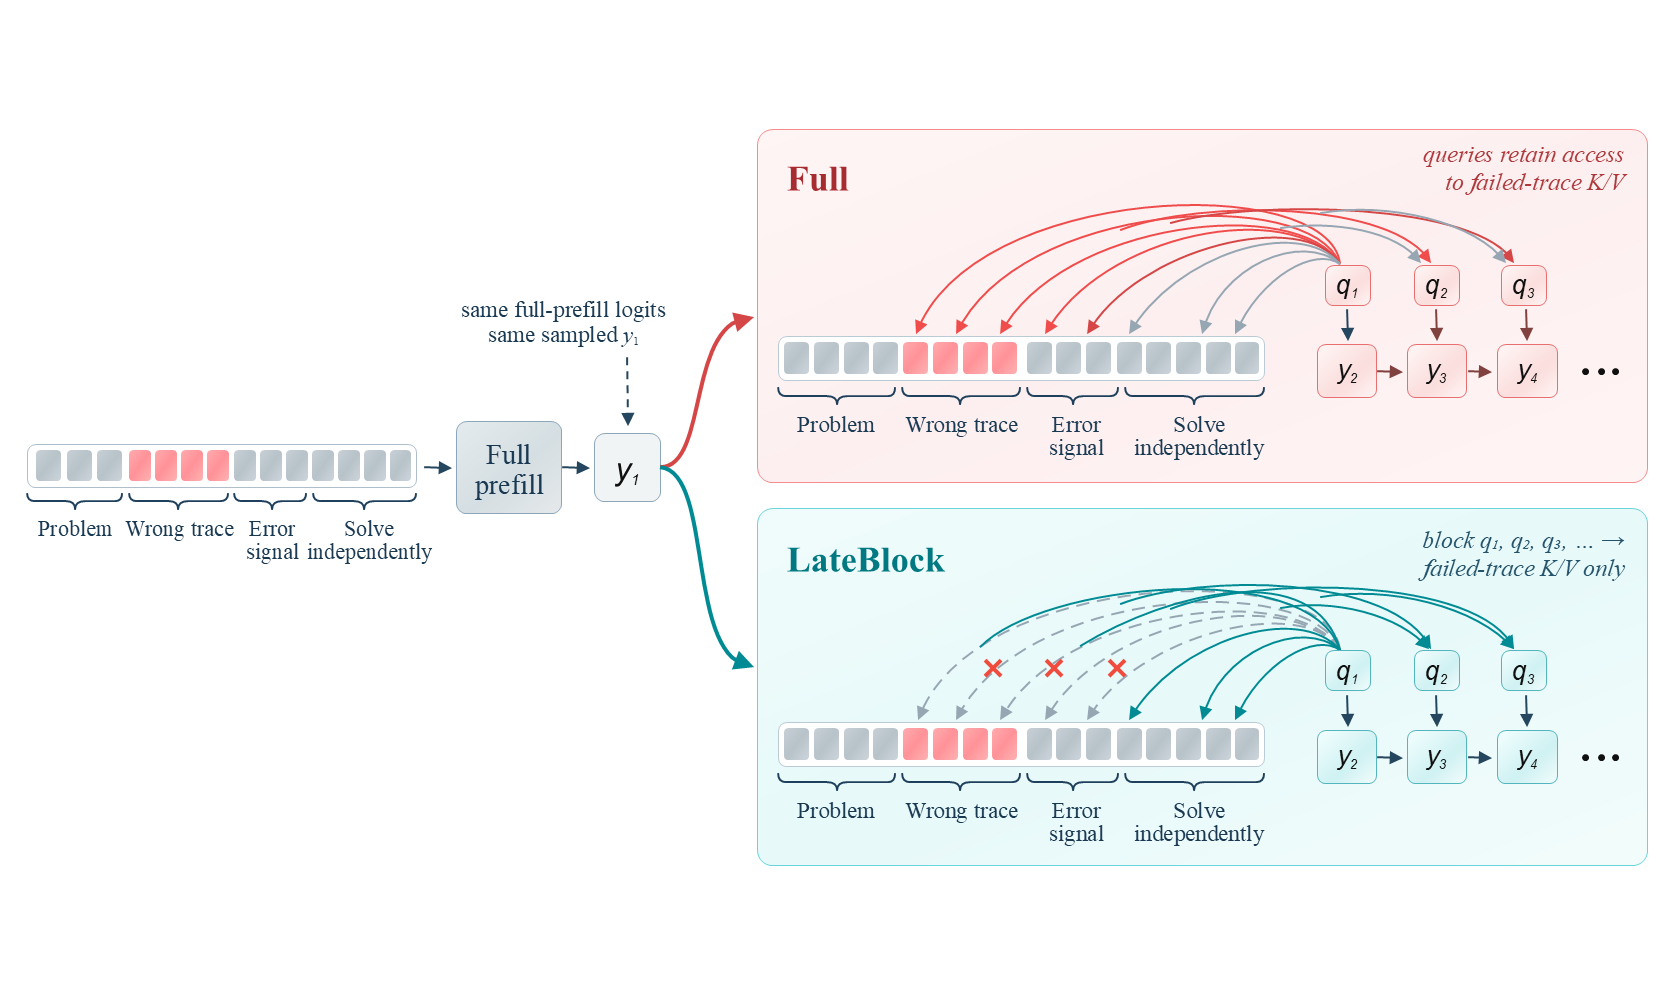
\includegraphics[width=\textwidth,trim=18bp 72bp 18bp 72bp,clip]{figure1_temp.png}
    \caption{Same-text intervention isolating continued access after full
    exposure. The prompt itself is unchanged. In \fullaccess{}, every generated query retains ordinary causal access to
    the known-wrong draft. In \lateblock{}, the complete prompt is processed with ordinary
    causal attention, and $y_1$ is sampled from the same full-prefill logits as
    in \fullaccess{}. Only then does blocking begin: the query at the $y_1$ position,
    which predicts $y_2$, is the first affected query. It and all subsequent
    generated queries cannot directly attend to the failed-draft key--value positions. Dashed arrows and crosses denote the
    removed attention edges. Access to the problem, error signal, and
    independent-solve instruction is preserved.}
    \label{fig:continued-access-overview}
\end{figure}

\noindent\textbf{Main Findings.}
On 23 selected Game24 questions, Qwen3-8B accuracy falls from 40/46 in clean context to 18/46 with a failed draft and explicit error feedback. Blocking only later direct access raises accuracy to 36/46, an effect of $+39.1$ percentage points [23.9, 54.3] (Section~\ref{sec:results}). This is the primary result: a substantial part of the observed loss depends on continued access even after full prefill exposure, while the interval and residual gap to clean context do not establish complete recovery.

The same directional pattern appears for Qwen3-32B and Gemma 4 E4B on a shared 15-question subset and for Qwen3-8B on two eight-question MATH source groups. On eight Game24 questions with verified correct history, however, blocking lowers accuracy from 16/16 to 13/16. Together, these results suggest that the effect of continued access depends on the quality of the retained history.

Finally, beginning the block earlier gives no consistent additional benefit. The late intervention is therefore sufficient for the observed recovery, even though other prompt and generated states may still carry information from the draft. We use access control as an identification tool: it tests the causal contribution of continued direct access after exposure. Error detection, a unique information pathway, and the deployment value of blocking require separate evidence.

\section{Access Intervention and Evaluation Setup}
\label{sec:setup}

Let a reasoning problem be $x$, and let $d=(d_1,\ldots,d_m)$ be a model-generated trajectory for the same problem that has been externally verified as incorrect. The evaluation prompt contains the problem, the complete text of $d$, an explicit signal that $d$ is incorrect, and an instruction to solve $x$ independently. Let $y=(y_1,\ldots,y_T)$ denote the new generated trajectory.

Under full causal attention, a generated query at position $q$ can attend prompt keys in the failed-draft span $D$. We intervene on the binary accessibility relation $A(q,k)$. \fullaccess{} preserves the ordinary causal mask:
\begin{equation}
    A_{\mathrm{full}}(q,k)=\mathbb{1}[k\leq q].
\end{equation}
Our primary intervention, \lateblock{}, preserves all prefill access and then blocks generated queries from attending to the draft. For a draft span $D=[s_d,e_d)$ and prompt length $L$,
\begin{equation}
    A_{\mathrm{late}}(q,k)
    = A_{\mathrm{full}}(q,k)\,\mathbb{1}[q<L \;\lor\; k\notin D].
    \label{eq:late}
\end{equation}
All prompt queries, including the full prefill, therefore use ordinary causal attention. The logits used to sample $y_1$ are also the ordinary full-prefill logits. Blocking first affects the next query after $y_1$ has been appended.

The secondary \pathblock{} diagnostic begins earlier, at the prompt suffix following the draft:
\begin{equation}
    A_{\mathrm{path}}(q,k)
    = A_{\mathrm{full}}(q,k)\,\mathbb{1}[q<e_d \;\lor\; k\notin D].
    \label{eq:path}
\end{equation}
This blocks post-draft prompt queries and generated queries from directly attending to $D$, while preserving computation within the draft itself. It tests intervention timing. Unblocked states may still carry draft-derived information. The equations display the rule for full causal layers. For a model with native sliding-window layers, we intersect the additional access restriction with that layer's native attention relation, preserving its ordinary computation wherever the intervention does not apply.

\subsection{Experimental conditions}

Table~\ref{tab:conditions} summarizes the four conditions used in the main experiment.

\begin{table}[t]
\caption{Experimental conditions. \fullaccess{}, \lateblock{}, and \pathblock{} share identical prompt text, token IDs, absolute positions, draft span, error signal, and sampling configuration.}
\label{tab:conditions}
\centering
\begin{tabular}{llll}
\toprule
Condition & History & Prefill access & Later draft access \\
\midrule
\clean{} & None & N/A & N/A \\
\fullaccess{} & Failed draft & Full & Full \\
\lateblock{} & Failed draft & Full & Blocked \\
\pathblock{} & Failed draft & Blocked after draft & Blocked \\
\bottomrule
\end{tabular}
\end{table}

Our primary estimands are
\begin{align}
    \Delta_{\mathrm{drag}} &= \operatorname{Acc}(\clean{})-\operatorname{Acc}(\fullaccess{}), \\
    \Delta_{\mathrm{access}} &= \operatorname{Acc}(\lateblock{})-\operatorname{Acc}(\fullaccess{}).
\end{align}
$\Delta_{\mathrm{drag}}>0$ denotes an observed loss from the failed-history prompt. The primary causal contrast is \lateblock{} versus \fullaccess{}: $\Delta_{\mathrm{access}}$ measures the accuracy change from removing later direct access at fixed initial exposure. A positive contrast represents recovery when the drag prerequisite holds. Its sampling uncertainty is reported separately. The secondary contrast between \pathblock{} and \lateblock{} probes whether beginning the block earlier improves recovery.

\subsection{Method}
\label{sec:method}

\paragraph{Same-text access intervention.}

For each problem--draft pair, we tokenize the complete prompt once and reuse its token IDs, positions, and draft span in \fullaccess{}, \lateblock{}, and \pathblock{}. The error label and decoding settings are also fixed, so \fullaccess{} and \lateblock{} differ only in later draft access. The mask changes logical attention edges while keeping the draft keys and values at their original positions. Invalid span or access metadata stops the request. Qwen uses vLLM with FlexAttention, while Gemma uses an eager Hugging Face implementation that preserves its hybrid attention layout. We analyze within-model contrasts because these backends are not bitwise equivalent. Backend-specific details, mask validation, and hash checks are reported in Appendix~\ref{app:details}.

\subsection{Experimental Design}
\label{sec:experiments}

\paragraph{Models and decoding.}

We evaluate Qwen3-8B, Qwen3-32B~\citep{qwen2025qwen3}, and Gemma 4 E4B~\citep{google2026gemma4}, each in its recorded thinking mode. Qwen3-8B is evaluated under all four conditions. The other models use \clean{}, \fullaccess{}, and \lateblock{}. Within each model, conditions share the same inference implementation, decoding configuration, and scorer. Decoding settings and random seeds are provided in Appendix~\ref{app:decoding}.

\paragraph{Game24.}

Game24 requires combining four input numbers with arithmetic operations to obtain 24, using each number exactly once. It provides executable correctness and a compact solution structure, and has been used to study deliberate LLM reasoning~\citep{yao2023tree}. We score the final expression for arithmetic correctness and input-multiset compliance.

We evaluate 23 questions with Qwen3-8B and a shared 15-question subset with the other targets, using two paired seeds per question. Baseline screening required two verified correct and two substantive incorrect trajectories, with one question retained under an earlier rule. Each question has one frozen failed draft, reused across target models where applicable. Intervention outcomes did not determine inclusion. Appendix~\ref{app:acquisition} details screening. Table~\ref{tab:coverage-sensitivity} in Appendix~\ref{app:coverage} reports eligibility and draft-content sensitivities.

\paragraph{Mathematical reasoning.}

As a cross-task check, we evaluate 16 MATH/MATH500 problems~\citep{hendrycks2021math} with Qwen3-8B, two seeds, and four conditions per problem. Eight MATH500 problems use Qwen3-1.7B source drafts, and eight MATH-train problems use Qwen3-4B source drafts. All drafts are verified substantive failures. We report the groups separately because problem source and draft-source model vary together. Scoring details are provided in Appendix~\ref{app:decoding}.

\paragraph{Clean comparator.}
Removing the entire failed-history block yields the \clean{} prompt. This changes both initial exposure and later access, providing a no-history reference. The primary controlled contrast is \lateblock{} versus \fullaccess{}, which holds prompt content and initial exposure fixed.

\paragraph{Correct-history specificity.}
To examine whether blocking helps regardless of history quality, we repeat the \lateblock{}--\fullaccess{} comparison with verified correct drafts on eight Game24 questions using Qwen3-8B. Correct drafts are selected without observing intervention outcomes, using character length for matching to failed drafts, and are explicitly labeled \texttt{CORRECT}. On these same eight questions and paired seeds, we define
\begin{align}
    \Delta_h &= \operatorname{Acc}_h(\lateblock{})-\operatorname{Acc}_h(\fullaccess{}),
    \quad h\in\{\mathrm{failed},\mathrm{correct}\}, \\
    \Delta_{\mathrm{specific}} &= \Delta_{\mathrm{failed}}-\Delta_{\mathrm{correct}}.
\end{align}
Here $\operatorname{Acc}_h$ denotes accuracy with history type $h$. The interaction measures dependence on history quality. It does not isolate truth value, because the drafts also differ in content and potentially other features.

\paragraph{Metrics and uncertainty.}

Accuracy is computed over all paired requests. Unresolved scores remain in the denominator and count as incorrect. We also report paired wrong-to-correct and correct-to-wrong transitions. The 95\% percentile intervals use 50,000 bootstrap resamples of questions, keeping both seeds for each question together. These intervals describe variation within the selected question set and do not account for uncertainty from question selection or study-design choices. Termination and score coverage are reported in Appendix~\ref{app:diagnostics}.

\section{Empirical Evaluation of Continued Access}
\label{sec:results}

\subsection{Failed reasoning remains harmful after explicit feedback}
\label{sec:residual-drag}

We first establish the prerequisite for interpreting an access effect as recovery. With Qwen3-8B, the failed-history prompt scores 18/46 versus 40/46 in clean context, despite the explicit incorrect-answer label and instruction to solve independently (Table~\ref{tab:game24}). The observed drag is 47.8 percentage points (95\% interval: 34.8 to 60.9). On the shared 15-question subset, Qwen3-32B and Gemma 4 E4B also show losses, respectively 36.7 points [16.7, 56.7] and 20.0 points [3.3, 33.3]. The comparison between \clean{} and \fullaccess{} establishes the phenomenon in these selected questions. It does not isolate the contribution of later access.

\subsection{Blocking continued access recovers most of the observed loss}
\label{sec:main-access}

\lateblock{} preserves the full prompt and its prefill computation, yet raises Qwen3-8B accuracy from 18/46 to 36/46. The 39.1-point access effect [23.9, 54.3] recovers most of the 47.8-point aggregate \clean{}--\fullaccess{} gap. Paired outcomes clarify the change: 21 trials move from wrong to correct, three from correct to wrong, 15 remain correct, and seven remain wrong. Figure~\ref{fig:question-recovery} shows how the gain is distributed across the selected questions: \lateblock{} yields more correct seeds on 15 questions, the same count on seven, and fewer on one. \lateblock{} is 8.7 points below \clean{}, with an interval of $[-23.9,4.3]$ points. This is not an equivalence test or evidence of complete restoration. Excluding question 381, whose failed draft also contains a correct intermediate alternative, leaves a 38.6-point effect [22.7, 54.5] over 22 questions. The main conclusion is unchanged when excluding the single question admitted under an earlier eligibility rule (Appendix~\ref{app:coverage}).

Because the conditions agree through full prefill and the first sampled token, the recovery cannot be explained solely by avoiding initial exposure to the failed trace. Continued direct access therefore remains behaviorally consequential after full exposure. Figure~\ref{fig:access-effects} places this primary effect alongside the additional model, task, and correct-history comparisons.

\begin{figure}[t]
    \centering
    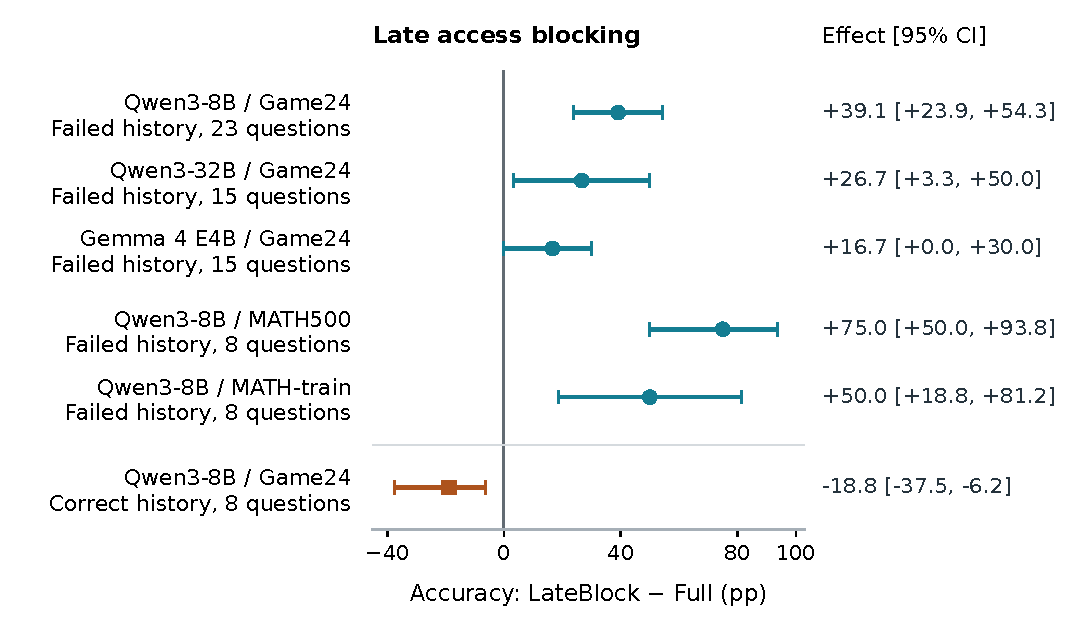
\includegraphics[width=\textwidth]{figure2_access_effects.pdf}
    \caption{Accuracy change from late access blocking. Points show \lateblock{} minus \fullaccess{} accuracy in percentage points for the indicated history type. Bars are 95\% percentile bootstrap intervals over questions, keeping the two seeds together. Qwen3-8B covers 23 Game24 questions. The other targets cover a shared 15-question subset, and the correct-history control covers eight questions. Each MATH row has eight questions and the Qwen3-8B target, with Qwen3-1.7B and Qwen3-4B source drafts for MATH500 and MATH-train, respectively. These rows are not a matched failed-versus-correct interaction. That comparison uses the same eight questions in Section~\ref{sec:specificity}. Unresolved scores count as incorrect.}
    \label{fig:access-effects}
\end{figure}

\begin{figure}[t]
    \centering
    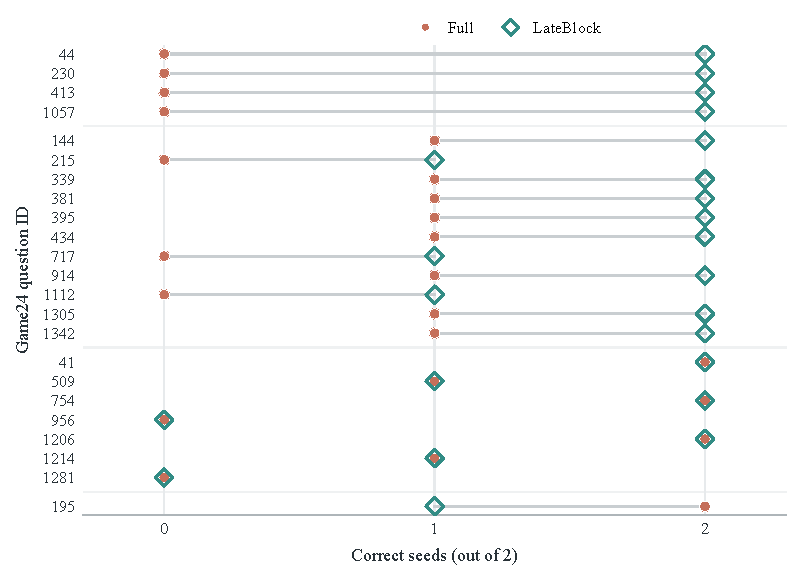
\includegraphics[width=0.92\textwidth]{figure3_question_level_recovery.pdf}
    \caption{Question-level recovery from late access blocking on Game24 with Qwen3-8B. Each row shows one of the 23 selected questions. Points denote the number of correct generations out of two paired seeds under full access (\fullaccess{}) and late access blocking (\lateblock{}). Lines connect the paired conditions for the same question. Rows are ordered by transition type, from the largest gains to declines, and by question ID within each type. The aggregate \fullaccess{}-to-\lateblock{} effect is $+39.1$ percentage points. The question-level view shows how recovery is distributed across the selected set.}
    \label{fig:question-recovery}
\end{figure}

\begin{table}[t]
\caption{Game24 accuracy with two seeds per condition: 23 questions for Qwen3-8B and a shared 15-question subset for the other targets. The primary contrast is \lateblock{} versus \fullaccess{}. Effects are percentage points. Brackets are 95\% intervals resampling questions. \pathblock{} and generation diagnostics appear in Appendix~\ref{app:diagnostics}.}
\label{tab:game24}
\centering
\begin{tabular}{lrrrr}
\toprule
Target & \clean{} & \fullaccess{} & \lateblock{} & $\Delta_{\mathrm{access}}$ [95\% CI] \\
\midrule
Qwen3-8B & 40/46 & 18/46 & 36/46 & $+39.1$ [$+23.9,+54.3$] \\
Qwen3-32B & 27/30 & 16/30 & 24/30 & $+26.7$ [$+3.3,+50.0$] \\
Gemma 4 E4B & 28/30 & 22/30 & 27/30 & $+16.7$ [$0.0,+30.0$] \\
\bottomrule
\end{tabular}
\end{table}

\subsection{The direction extends across target models and implementations}
\label{sec:target-models}

On the shared 15 questions and source drafts, Qwen3-8B gains 46.7 points [26.7, 66.7]. Qwen3-32B gains 26.7 points [3.3, 50.0] from \lateblock{} versus \fullaccess{}, with 11 improvements and three harms. Gemma 4 E4B gains 16.7 points [0.0, 30.0], with six improvements and one harm. The Gemma interval touches zero. These results show the same directional pattern with different magnitudes and uncertainty. The experiment is not designed to support conclusions about scaling with model size.

Qwen uses the vLLM/FlexAttention implementation, while Gemma uses a separate eager Hugging Face implementation that preserves its native hybrid attention. Observing the same direction in both provides a robustness check beyond one custom backend. Since architecture and implementation change together, it does not isolate backend effects or establish cross-backend equivalence. Generation termination and unresolved-score counts are reported in Appendix~\ref{app:diagnostics}.

\subsection{Blocking can harm correct history}
\label{sec:specificity}

Does late blocking help because the retained history is wrong, or could disrupting attention to any prior attempt improve performance? To examine this distinction, we apply the same intervention to verified correct history on eight Game24 questions with the same Qwen3-8B target. Full access scores 16/16, while late blocking scores 13/16: a $-18.8$-point effect [${-37.5},{-6.2}$]. All three discordant pairs favor full access. Access to these correct drafts is useful in the observed sample, so blocking has no unconditional advantage.

The failed-history access effect on these \emph{same eight questions} is $+37.5$ points. The matched difference in differences is therefore $+56.2$ points [${+37.5},{+75.0}$], rather than a comparison with the full 23-question effect. One blocked correct-history output is length-truncated and unresolved. Scoring it as correct still yields a $+50.0$-point interaction. Correct and failed histories differ in content, may differ in length, and receive different truthful feedback labels. The interaction supports dependence on history quality, but it does not isolate truth value or rule out all generic effects of attention disruption.

\subsection{The direction also appears in longer-form mathematical reasoning}
\label{sec:math-replication}

MATH provides a cross-task check under longer-form reasoning (Table~\ref{tab:math}). Both source groups show the drag prerequisite $\operatorname{Acc}(\clean{})>\operatorname{Acc}(\fullaccess{})$ and a positive access effect: 75.0 points [50.0, 93.8] for MATH500/Qwen3-1.7B drafts and 50.0 points [18.8, 81.2] for MATH-train/Qwen3-4B drafts. The groups differ simultaneously in source questions and draft-source model. Their contrast cannot identify either a source-model or draft-length mechanism.

\begin{table}[t]
\caption{Qwen3-8B target on MATH: eight questions per source group, two seeds per condition. Accuracy counts all requests. Unresolved scores count incorrect.}
\label{tab:math}
\centering
\begin{tabular}{lrrrr}
\toprule
Source / draft model & \clean{} & \fullaccess{} & \lateblock{} & $\Delta_{\mathrm{access}}$ [95\% CI] \\
\midrule
MATH500 / Qwen3-1.7B & 16/16 & 2/16 & 14/16 & $+75.0$ [$+50.0,+93.8$] \\
MATH-train / Qwen3-4B & 7/16 & 0/16 & 8/16 & $+50.0$ [$+18.8,+81.2$] \\
\bottomrule
\end{tabular}
\end{table}

Termination is less balanced than in Game24: of 128 MATH generations, 114 reach EOS, 14 stop at the length limit, and 13 scores are unresolved. MATH-train \lateblock{} and \pathblock{} have 4/16 and 6/16 length stops, respectively, versus none in \fullaccess{}. The contrasts thus concern scored success under the fixed generation budget and can reflect changes in both answer content and completion. They provide a directional cross-task check under longer-form reasoning, but do not establish a correctness effect independent of termination. Appendix~\ref{app:diagnostics} gives the condition-level counts.

\subsection{Earlier blocking provides no consistent additional benefit}
\label{sec:timing}

\pathblock{} tests whether blocking post-draft prompt queries also improves on late blocking (Table~\ref{tab:r4}, Appendix~\ref{app:diagnostics}). On Game24 with Qwen3-8B, it scores 35/46 versus \lateblock{}'s 36/46, giving $\operatorname{Acc}(\pathblock{})-\operatorname{Acc}(\lateblock{})=-2.2$ points [${-17.4},{+13.0}$]. The corresponding MATH contrasts are $+6.2$ points [${-12.5},{+25.0}$] and $-12.5$ points [${-43.8},{+12.5}$]. None shows a consistent additional benefit. These timing results constrain the conclusion: the observed recovery does not require the earlier intervention, and the data do not identify all mediated paths through which draft information may propagate.

\section{Analysis}
\label{sec:discussion}

\subsection{What the access contrast identifies}
The comparison between \fullaccess{} and \lateblock{} shows that processing a failed trace does not fully determine its effect on the next solution. Even after identical prefill computation and the same first sampled token, changing later direct access changes accuracy. Continued direct access therefore makes a causal contribution under the evaluated conditions. The error feedback is supplied externally, so this result concerns the model's response to known failure rather than its ability to recognize an error.

The clean baseline answers a complementary question. Comparing \clean{} with \fullaccess{} establishes a loss associated with the failed-history prompt, but changes both initial processing and later access. Comparing \lateblock{} with \fullaccess{} holds initial processing fixed and intervenes on later access. Their effect sizes are therefore not an additive decomposition of contextual drag into exposure and access components. Recovery of much of the clean-context gap does not measure the fraction of erroneous information removed from the model.

Across the 46 Qwen3-8B Game24 pairs, late blocking changes 21 incorrect outputs to correct ones and three correct outputs to incorrect ones. The remaining pairs contain 15 shared successes and seven shared failures (Table~\ref{tab:game24-per-question}). Figure~\ref{fig:question-recovery} shows their distribution across questions. The average benefit thus coexists with individual losses and persistent failures.

\subsection{History dependence of the access effect}
The correct-history comparison tests whether the benefit extends to useful prior reasoning. On the same eight questions, the failed-history access effect is $+37.5$ points, whereas the correct-history effect is $-18.75$ points. The resulting interaction is $+56.2$ points (Section~\ref{sec:specificity}). Comparing the same questions avoids attributing the reversal to a difference in question composition. The small control set nevertheless limits how precisely this dependence can be characterized.

Within each history type, \fullaccess{} and \lateblock{} receive the same feedback label. Across history types, both the draft and its truthful label change. The interaction therefore concerns the draft--feedback combination, rather than correctness as an isolated property. Matching drafts by character length does not equate their token counts, reasoning paths, or useful intermediate content. The reversal motivates selective access, but the final-answer label alone cannot locate every useful or harmful step in a draft.

An output-level audit on these eight questions provides a complementary behavioral measure. After normalization, the extracted final expression exactly repeats the frozen failed expression in 9/16 \fullaccess{} outputs, 2/16 \lateblock{} outputs, and 1/16 \pathblock{} outputs. Reduced reuse accompanies improved accuracy, connecting the access intervention to a visible change in the final answer. This measure does not classify algebraically equivalent expressions or shared reasoning routes. It therefore describes output persistence without establishing an internal copying mechanism or an estimate for all 23 questions.

\subsection{Scope of the intervention}
\lateblock{} preserves full prefill computation, so unblocked prompt states can carry draft-derived information into generation. Retaining these possible indirect routes makes the comparison informative about access after exposure. Once generation proceeds, the conditions can produce different tokens and states. The measured effect includes these downstream consequences of changing the access rule across layers and generation steps.

Blocking draft keys also changes the set of positions over which attention is normalized. The relative contribution of the problem, feedback, and generated prefix can therefore change even though their keys remain available. Improved accuracy may reflect reduced use of misleading draft information, increased use of other context, or both. These changes are consequences of the access intervention. The comparison identifies their combined effect on accuracy without separating their internal contributions. A matched irrelevant-history control could test whether the benefit depends on the draft's relationship to the current problem.

\pathblock{} additionally blocks post-draft prompt queries, changing the suffix computation during prefill as well as later access. Its comparison with \lateblock{} evaluates this earlier-starting access policy. Table~\ref{tab:r4} shows no consistent additional gain, although the intervals allow both benefits and harms. Recovery with \lateblock{} establishes that the earlier restriction is unnecessary for the observed improvement. The comparison does not establish equivalence between the policies or show that initial processing is irrelevant.

Selective-access experiments could compare useful and erroneous steps while controlling span length, position, and feedback. Spans would need to be selected without consulting later outcomes. Practical use would also require evaluating span selection, runtime, memory, and task performance.

\section{Related Work}

\paragraph{Refinement and contextual drag.}
Self-refinement and Reflexion retain earlier outputs or feedback to guide later attempts~\citep{madaan2023selfrefine,shinn2023reflexion}. \citet{cheng2026contextualdrag} show that failed in-context attempts can lower performance, induce structurally related errors, and persist despite explicit verification. They also study denoising and targeted fine-tuning. We take contextual drag as the starting point and examine whether continued direct access contributes after the failed trajectory has already been processed.

\paragraph{Prior attempts across turns.}
Studies of multi-turn interaction report over-reliance on early answers and persistence of errors in later assistant responses~\citep{laban2026lostconversation,huang2026ownwords}. Those settings change the information revealed over time or filter what history is processed. Our same-problem comparison holds the prompt and initial exposure fixed while varying later direct access.

\paragraph{Context management and causal interventions.}
PagedAttention organizes KV-cache storage for efficient serving, while H$_2$O studies KV-cache eviction~\citep{kwon2023pagedattention,zhang2023h2o}. MEMENTO studies how LLMs manage their textual context~\citep{kontonis2026memento}. Causal tracing, activation patching, and path patching intervene on internal computations to localize effects~\citep{meng2022causaltracing,zhang2024activationpatching,goldowsky2023pathpatching,dura2026sequentialpatching}. Our attention mask preserves prompt tokens, full prefill, and first-token computation while controlling later access to a designated prompt span. FlexAttention supplies the programmable mask interface~\citep{dong2025flexattention}. Our contribution is the controlled access comparison enabled by this interface.

\section{Limitations}

The 23 Game24 questions are selected for mixed baseline outcomes, and eight came from the completed portion of a screening run that ended early for runtime reasons, leaving ten candidates incomplete. The cutoff could therefore favor candidates with shorter or faster screening trajectories. The protocol also developed across collection batches, and the bootstrap intervals do not capture this selection or adaptation. These restrictions limit the population to which the reported effect sizes generalize. Broader coverage of independently selected questions is needed to characterize generalization beyond this selected sample.

The intervention additionally assumes externally verified incorrect drafts and known token spans. The additional models vary in both architecture and inference implementation, so their agreement supports robustness but does not explain model differences. Logical blocking leaves allocated KV tensors and information in unblocked states intact. MATH has condition-dependent termination and unresolved answers, and the correct-history subset does not match failed histories on every feature. The results therefore do not establish a sole information pathway, a scaling law, or a universally useful mitigation.

\section{Conclusion}

Continued direct access to failed reasoning can affect a new solution after full initial exposure and explicit error feedback. Our same-text intervention identifies this contribution while preserving prefill computation and the first sampled token. Late blocking recovers substantial accuracy on the selected Game24 set, with the same directional pattern in additional models and MATH settings. Blocking correct history instead harms performance, showing that the effect depends on the retained history and its feedback. These findings motivate studying when selective access can preserve useful prior work while limiting interference from failed reasoning.

\subsection*{Reproducibility statement}
The paper specifies the model and inference configurations, random seeds, and scoring rules. Appendix~\ref{app:details} describes the intervention semantics, implementation checks, and prompt templates. The supplementary artifact contains implementation and scoring code, all 524 experimental records with infrastructure metadata removed, and an evidence manifest linking these records to the reported summaries. Its analysis scripts reconstruct the reported statistics and result figures, including question-level and seed-level tables.

\subsection*{AI use statement}
Generative AI tools assisted with code development, debugging, discussions of experimental design, experiment documentation, literature discovery, result interpretation, and language editing. Numerical claims are tied to persisted results and auditable analysis scripts. The submitting authors are responsible for the final manuscript, its claims, and the associated artifacts.

\bibliography{contextual_drag_continued_access}
\bibliographystyle{iclr2027_conference}

\clearpage
\appendix

\section{Intervention and Experimental Details}
\label{app:details}

\paragraph{Condition names and artifact IDs.}
The display names \clean{}, \fullaccess{}, \lateblock{}, and \pathblock{} correspond to internal artifact IDs \texttt{R0}, \texttt{R2}, \texttt{R3}, and \texttt{R4}, respectively. These IDs are retained in code and persisted results. Unless explicitly labeled as a correct-history control, \fullaccess{}, \lateblock{}, and \pathblock{} use a failed draft with explicit error feedback.


\subsection{Access semantics}

Table~\ref{tab:access-semantics} distinguishes KV allocation from attention access during prefill and decoding.

\begin{table}[h]
\caption{Operational semantics of the access modes. ``Allocated'' means that the KV tensors remain present in memory. The intervention controls whether the corresponding logical attention edges participate.}
\label{tab:access-semantics}
\centering
\begin{tabular}{llll}
\toprule
Mode & Draft KV allocated & Prefill & Decode \\
\midrule
\fullaccess & Yes & Ordinary causal & Ordinary causal \\
\lateblock & Yes & Ordinary causal & Draft keys blocked \\
\pathblock & Yes & Block after draft end & Draft keys blocked \\
\bottomrule
\end{tabular}
\end{table}

\lateblock{}'s first sampled token uses the same full-prefill logits as \fullaccess{}. In implementation terms, the first blocked query has logical position equal to the prompt length. \pathblock{} starts blocking at the end of the draft span and therefore also affects the prompt suffix following the draft. Neither mode physically compacts KV storage or renumbers token positions.

\subsection{Implementation validation checklist}

Before a scientific run, we verify:
\begin{enumerate}
    \item equality of \fullaccess{}, \lateblock{}, and \pathblock{} prompt text, token IDs, length, positions, and hashes;
    \item validity and minimum-span coverage of the persisted draft interval;
    \item agreement of request-specific paged logical masks with a dense reference;
    \item first-token agreement between full and late-block conditions in deterministic checks;
    \item zero output change under mutations confined to keys blocked by the tested path mask in targeted greedy checks;
    \item fail-closed behavior for missing metadata, unsupported layouts, or version mismatch.
\end{enumerate}

\subsection{Decoding, scoring, and the clean comparator}
\label{app:decoding}

We use temperature $0.6$, top-$p$ $0.95$, top-$k$ $20$, and a 32,768-token context limit. The paired Game24 seeds are 927001 and 927002. The MATH seeds are 930001 and 930002. All \clean{} outputs are generated for the reported comparisons, without substituting screening outputs. For MATH, the frozen scorer compares the last complete boxed answer with the reference answer.

Removing the complete failed-history block, including its label and delimiters, yields the \clean{} user content under the recorded chat wrapper. This equivalence was audited for all 32 MATH \clean{} requests.

\subsection{Draft acquisition and leakage control}
\label{app:acquisition}

The 23 Game24 questions are distinct, and each has one frozen failed draft. Baseline screening determines draft correctness before intervention evaluation. Manual review distinguishes substantive failures from format-only errors, incomplete trajectories, and scorer failures. Twenty-two questions meet the final two-correct/two-failure rule. ID 41 was admitted under an earlier rule. Eight questions were retained from the completed portion of a larger screening run that ended early for runtime reasons. The set was collected in successive batches and is treated as one selected sample, not as a preregistered replication. We transfer only source models' visible final responses, without private thinking traces. No intervention response is used to relabel its frozen source draft.

\subsection{Statistical reporting}

For each condition and contrast, we report raw numerators and denominators, accuracy, paired transitions, question-cluster bootstrap intervals, EOS rate, score coverage, and length termination. We resample questions, keeping both seed-level observations together. Effects are descriptive for the selected questions. Intervals are not adjusted for multiple contrasts and do not incorporate the uncertainty introduced by sample selection or study-design choices.

\section{Generation Diagnostics and Earlier Blocking}
\label{app:diagnostics}

Table~\ref{tab:diagnostics} reports all 524 completed scientific requests used in the paper. EOS and scoring coverage are distinct: one Gemma \lateblock{} output reaches EOS but has an unresolved score, whereas four length-stopped outputs across the full dataset have an extracted answer scored incorrect. All length-stopped outputs are either scored incorrect or unresolved. No records are dropped because of termination or parsing outcomes.

% Generated by audit_iclr2027_revision_20260925.py
\begin{table}[H]
\centering
\caption{All completed requests in the paper. Correctness uses persisted benchmark scores; unresolved answers count as incorrect. Termination is reported separately. MATH rows use the Qwen3-8B target.}
\label{tab:diagnostics}
\begin{tabular}{llrrrr}
\toprule
Task / target & Condition & Correct & EOS & Length & Unresolved \\
\midrule
Game24 / Qwen3-8B & \clean{} & 40/46 & 44 & 2 & 1 \\
 & \fullaccess{} & 18/46 & 46 & 0 & 0 \\
 & \lateblock{} & 36/46 & 44 & 2 & 1 \\
 & \pathblock{} & 35/46 & 45 & 1 & 0 \\
\addlinespace[3pt]
Game24 / Qwen3-32B & \clean{} & 27/30 & 30 & 0 & 0 \\
 & \fullaccess{} & 16/30 & 30 & 0 & 0 \\
 & \lateblock{} & 24/30 & 30 & 0 & 0 \\
\addlinespace[3pt]
Game24 / Gemma 4 E4B & \clean{} & 28/30 & 30 & 0 & 0 \\
 & \fullaccess{} & 22/30 & 30 & 0 & 0 \\
 & \lateblock{} & 27/30 & 30 & 0 & 1 \\
\addlinespace[3pt]
MATH500 / Qwen3-8B & \clean{} & 16/16 & 16 & 0 & 0 \\
 & \fullaccess{} & 2/16 & 15 & 1 & 1 \\
 & \lateblock{} & 14/16 & 15 & 1 & 1 \\
 & \pathblock{} & 15/16 & 15 & 1 & 1 \\
\addlinespace[3pt]
MATH-train / Qwen3-8B & \clean{} & 7/16 & 15 & 1 & 1 \\
 & \fullaccess{} & 0/16 & 16 & 0 & 0 \\
 & \lateblock{} & 8/16 & 12 & 4 & 3 \\
 & \pathblock{} & 6/16 & 10 & 6 & 6 \\
\addlinespace[3pt]
Correct history / Qwen3-8B & \fullaccess{} & 16/16 & 16 & 0 & 0 \\
 & \lateblock{} & 13/16 & 15 & 1 & 1 \\
\addlinespace[3pt]
\bottomrule
\end{tabular}
\end{table}


Table~\ref{tab:r4} compares \pathblock{} with both \fullaccess{} and \lateblock{}, separating recovery under earlier blocking from its additional effect relative to late blocking.

\begin{table}[H]
\centering
\caption{Earlier-blocking diagnostic with the Qwen3-8B target. The \pathblock{} column reports correct counts. We define $\Delta_{\mathrm{path}}=\operatorname{Acc}(\pathblock{})-\operatorname{Acc}(\fullaccess{})$ and $\Delta_{\mathrm{early}}=\operatorname{Acc}(\pathblock{})-\operatorname{Acc}(\lateblock{})$. Effects are percentage points with question-cluster 95\% bootstrap intervals.}
\label{tab:r4}
\begin{tabular}{lrrr}
\toprule
Task & \pathblock{} & $\Delta_{\mathrm{path}}$ [95\% CI] & $\Delta_{\mathrm{early}}$ [95\% CI] \\
\midrule
Game24 & 35/46 & $+37.0$ [$+21.7,+52.2$] & $-2.2$ [$-17.4,+13.0$] \\
MATH500 & 15/16 & $+81.2$ [$+56.2,+100.0$] & $+6.2$ [$-12.5,+25.0$] \\
MATH-train & 6/16 & $+37.5$ [$+12.5,+75.0$] & $-12.5$ [$-43.8,+12.5$] \\
\bottomrule
\end{tabular}
\end{table}

\section{Prompts}

The prompt builder uses the following Game24 user-content template, with the two bracketed fields replaced by the frozen pair. Line wrapping of the final instruction below is typographic. The builder joins it into one line. The model-specific chat template surrounds this content.
\begin{verbatim}
Original problem:
[problem]

The following draft has an INCORRECT final answer.
-- beginning of the draft --
[draft]
-- end of the draft --

Solve the original problem independently and provide a
complete solution. You do not need to evaluate or refer
to any preceding draft. Conclude with an expression using
the original four numbers exactly once in \boxed{}.
\end{verbatim}
For MATH, the last sentence is ``Conclude with your final answer in \textbackslash boxed\{\}.'' \clean{} omits the entire history block, including the incorrect-answer label and delimiters. The correct-history control changes the label to \texttt{CORRECT} and inserts a verified correct draft.

\section{Complete Question-Level Results}

Table~\ref{tab:game24-per-question} gives all Game24 question-level counts. \fullaccess{}/\lateblock{} prompt hashes, input-token hashes, draft spans, and first generated tokens match for all 46 Qwen3-8B paired units and all 30 units per other target model. The Qwen3-8B \fullaccess{}/\lateblock{} transitions are 21 wrong-to-correct, three correct-to-wrong, 15 both correct, and seven both wrong. For Qwen3-32B they are 11, three, 13, and three. For Gemma 4 E4B they are six, one, 21, and two.

% Generated from persisted scorer decisions by build_iclr2027_evidence_20260925.py
\begin{table}[!t]
\centering
\caption{Game24 correct counts per question. Each count is out of two seeds. Counts are ordered as \clean{}, \fullaccess{}, \lateblock{}, and \pathblock{} for Qwen3-8B (23 questions). The other models cover the shared 15-question subset and report the first three conditions in the same order. A dash denotes an unevaluated model--question combination.}
\label{tab:game24-per-question}
\begin{tabular}{rccc}
\toprule
Question & Qwen3-8B & Qwen3-32B & Gemma 4 E4B \\
\midrule
41 & 2/2/2/2 & 2/1/2 & 2/2/2 \\
44 & 2/0/2/2 & 1/2/2 & 2/1/2 \\
144 & 2/1/2/2 & --- & --- \\
195 & 2/2/1/2 & --- & --- \\
215 & 2/0/1/1 & --- & --- \\
230 & 2/0/2/2 & 2/1/1 & 2/2/2 \\
339 & 2/1/2/2 & 2/2/2 & 2/2/2 \\
381 & 2/1/2/2 & --- & --- \\
395 & 2/1/2/2 & --- & --- \\
413 & 1/0/2/1 & 2/0/1 & 2/1/0 \\
434 & 2/1/2/2 & --- & --- \\
509 & 2/1/1/1 & 2/1/2 & 2/1/2 \\
717 & 1/0/1/1 & 2/2/1 & 2/2/2 \\
754 & 2/2/2/2 & 2/1/2 & 2/1/2 \\
914 & 2/1/2/2 & 2/1/1 & 2/2/2 \\
956 & 2/0/0/1 & 1/1/1 & 2/1/2 \\
1057 & 1/0/2/0 & 1/0/2 & 2/2/2 \\
1112 & 2/0/1/2 & 2/0/2 & 2/2/2 \\
1206 & 2/2/2/2 & --- & --- \\
1214 & 1/1/1/2 & 2/1/2 & 2/1/2 \\
1281 & 1/0/0/0 & --- & --- \\
1305 & 1/1/2/0 & 2/1/2 & 1/0/1 \\
1342 & 2/1/2/2 & 2/2/1 & 1/2/2 \\
\bottomrule
\end{tabular}
\end{table}



\section{Coverage and Draft-Content Sensitivity}
\label{app:coverage}

Table~\ref{tab:coverage-sensitivity} summarizes how the pooled access effect changes when either the mixed-content draft or the earlier-rule question is excluded.

The eight questions from the completed screening prefix contribute all 64 planned outputs, using fresh \clean{} generations and the same seeds, decoding, and scoring as the earlier evaluation. \clean{}, \fullaccess{}, \lateblock{}, and \pathblock{} score 15/16, 8/16, 12/16, and 13/16. Their \lateblock{}--\fullaccess{} effect is 25.0 points [0.0, 43.8], with five wrong-to-correct and one correct-to-wrong transition. Thus this extension agrees in direction but has a smaller and less precise effect than the shared 15-question subset. Its two length-stopped outputs are scored incorrect and remain in the denominators. All 64 extracted final expressions were checked with exact arithmetic and input-multiset verification, agreeing with their persisted scores.

Before generation, we specified a sensitivity analysis excluding question 381 because its fixed source draft contains a correct intermediate expression but explicitly selects an invalid final expression. Excluding it leaves \clean{}, \fullaccess{}, \lateblock{}, and \pathblock{} at 38/44, 17/44, 34/44, and 33/44 over 22 questions. The access effect remains 38.6 points [22.7, 54.5]. Within the eight-question extension alone, exclusion leaves 13/14, 7/14, 10/14, and 11/14, with an access effect of 21.4 points [$-7.1$, 42.9]. This smaller subset remains uncertain. The pooled conclusion does not depend on the mixed-content draft. No draft was replaced after observing intervention outcomes.

As a separate eligibility sensitivity, excluding question 41, which was admitted under an earlier rule, leaves 22 questions with \fullaccess{}/\lateblock{} accuracy of 16/44 and 34/44. The access effect is +40.9 points (95\% question-cluster bootstrap interval: [+25.0,+56.8]), close to the pooled estimate. This confirms that the main conclusion does not depend on the single earlier-rule inclusion.

\begin{table}[H]
\caption{Sensitivity of the Qwen3-8B Game24 access effect to question eligibility and draft content. Each question contributes two paired seeds. Intervals are 95\% question-cluster percentile bootstrap intervals.}
\label{tab:coverage-sensitivity}
\centering
\begin{tabular}{lrrrr}
\toprule
Analysis & Questions & \fullaccess{} & \lateblock{} & $\Delta_{\mathrm{access}}$ [95\% CI] \\
\midrule
Pooled main sample & 23 & 18/46 & 36/46 & $+39.1$ [$+23.9,+54.3$] \\
Exclude question 381 & 22 & 17/44 & 34/44 & $+38.6$ [$+22.7,+54.5$] \\
Exclude question 41 & 22 & 16/44 & 34/44 & $+40.9$ [$+25.0,+56.8$] \\
\bottomrule
\end{tabular}
\end{table}

\section{Data Availability}

Public benchmark items retain their original licenses and provenance. Model weights are referenced by immutable model identifiers and are not redistributed.

\end{document}
